\section{Dini Permata Putri | 1174053}
\subsection{Teori}
\begin{enumerate}

\item Apa itu fungsi file csv, jelaskan sejarah dan contoh\\
jawab : file CSV atau Comma Separated Value seperti namanya berisi teks data yang tiap datanya dipisahkan dengan tanda koma. Sebagai gambaran, sebuah file CSV bisa berisi data berikut ini :\\
HeaderA, HeaderB, HeaderC\\
RowA1, RowB1, RowC1\\
RowA2, RowB2, RowC2\\
Jika kita membuat sebuah file di Excel dan menyimpannya dalam format CSV, maka file tersebut dibuka di Notepad maka akan terlihat isi file yang kurang lebih formatnya sama seperti di atas.\\

\item Aplikasi-aplikasi apa saja yang bisa menciptakan file csv?\\
jawab : microsoft office, dll.\\

\item Jelaskan bagaimana cara menulis dan membaca file csv di excel atau spreadsheet\\
jawab : 1. Buka MS Excel Anda\\
2. Klik Data > Get External Data > From Text\\ 
3. Akan muncul Text Import Wizard, arahkan pada file csv yang ingin anda buka > Open.\\
4. Setelah File terbuka, akan muncul Text Import Wizard\\
Step 1 –> Pilih Delimited, Kemudian Next (Di sini, bisa juga menentukan baris awal yang akan di import)\\
Step 2 –> Centrang pada Tab dan Comma (Atau sesuai pengaturan File Anda) > Next\\
Step 3 –> Atur Format data pada tiap kolom yang tampil dan klik Finish\\

\item Jelaskan sejarah library csv\\
jawab : Jaringan perpustakaan digital pertama di Indonesia mulai beroperasi pada bulan Juni 2001.  Jaringan Perpustakaan Digital tersebut itu bernama IndonesiaDLN (Digital Library Network).  IndonesiaDLN diprakarsai oleh Knowledge Management Research Group (KMRG) Institut Teknologi Bandung (ITB) yang merintis pembuatan jaringan perpustakaan digital (digital library network) antar lembaga pendidikan tinggi.  Jaringan pustaka digital bertujuan mempermudah kalangan akademik dan masyarakat umum untuk mengakses hasil penelitian, tugas akhir mahasiswa, tesis maupun disertasi. Dana awal pengembangan jaringan berasal dari Singapura sebanyak 60.000 dolar Kanada, dan dari Yayasan Litbang Telekomunikasi dan Teknologi Informasi (YLTI) sebanyak Rp 150 juta. \\

Pada awal berdirinya, lembaga yang bergabung dalam jaringan pustaka digital IndonesiaDLN antara lain Proyek Pengembangan Universitas Indonesia Timur, LIPI Jakarta, Universitas Brawijaya Malang, Universitas Muhammadiyah Malang, Lembaga Penelitian ITB, Pasca Sarjana ITB, serta Computer Network Research Group (CNRG).\\

Ketua KMRG saat itu sekaligus sebagai penggagas IndonesiaDLN Ismail Fahmi menjelaskan bahwa ide dasar pengembangan pustaka digital bahwa hasil pemikiran dan penelitian harus bisa dipertukarkan (share) dan diakses secara cepat dan mudah. Copyright untuk tugas akhir maupun penelitian pada dasarnya termasuk public domain kecuali yang terikat pada perjanjian dengan industri atau dalam persiapan untuk mendapatkan hak paten. IndonesiaDLN bertujuan agar hasil-hasil penelitian dari perguruan tinggi maupun lembaga penelitian bisa diakes dari manapun di seluruh penjuru dunia dapat diakses secara mudah dan murah dalam bentuk digital, tanpa memerlukan biaya transportasi maupun fotokopi yang biasanya harus dengan mengeluarkan biaya cukup tinggi.\\

Gagasan pembentukan jaringan perpustakaan nasional ini bermula dari peluncuran situs Ganesha Digital Library/GDL (perpustakaan digital milik ITB) Oktober 2000. Sekitar 20 institusi kemudian terlibat dalam proyek jaringan perpustakaan ini. Beberapa server individu juga ikut menyebarkan informasinya melalui GDL, seperti Onno W. Purbo, Budi Rahardjo, dan Ismail Fahmi.\\

Jaringan pustaka digital ini merupakan satu dari beberapa produk KMRG. Produk lainnya adalah Ganesha digital library, software untuk otomatisasi perpustakaan (GNU-Lib) serta software untuk katalog database perpustakaan\\
(http://isisnetwork.lib.itb.ac.id).\\

Menurut Sekjen IndonesiaDLN,  Ismail Fahmi, jaringan perpustakaan digital ini berfungsi sebagai terminal dari berbagai server di Indonesia yang menyediakan informasi ilmu pengetahuan. Misi jaringan ini adalah mengelola ilmu pengetahuan yang dimiliki bangsa Indonesia, dalam satu jaringan yang terdistribusi dan terbuka.\\

\item Jelaskan sejarah library pandas\\
jawab : engembang Wes McKinney mulai mengerjakan pandas pada 2008 ketika di AQR Capital Management karena kebutuhan akan alat kinerja tinggi yang fleksibel untuk melakukan analisis kuantitatif pada data keuangan. Sebelum meninggalkan AQR, dia bisa meyakinkan manajemen untuk mengizinkannya membuka sumber perpustakaan.\\

Pegawai AQR lainnya, Chang She, bergabung dengan upaya ini pada 2012 sebagai kontributor utama kedua ke perpustakaan.\\

Pada 2015, panda ditandatangani sebagai proyek NumFOCUS yang disponsori secara fiskal, sebuah badan amal nirlaba 501 (c) (3) di Amerika Serikat.\\

\item Jelaskan fungsi-fungsi yang terdapat di library csv\\
jawab : Jika kita membuat sebuah file di Excel dan menyimpannya dalam format CSV, maka file tersebut dibuka di Notepad maka akan terlihat isi file yang kurang lebih formatnya sama seperti di atas.\\

\item Jelaskan fungsi-fungsi yang terdapat di library pandas\\
jawab : dapat mengolah suatu data dan mengolahnya seperti join, distinct, group by, agregasi, dan teknik seperti pada SQL. Hanya saja dilakukan pada tabel yang dimuat dari file ke RAM.\\

Pandas juga dapat membaca file dari berbagai format seperti .txt, .csv, .tsv, dan lainnya. Anggap saja Pandas adalah spreadsheet namun tidak memiliki GUI dan punya fitur seperti SQL.\\
\end{enumerate}

%%%%%%%%%%%%%%%%%%%%%%%%%%%%%%%%%%%%%%%%%%%%%%%%%%%%%%%%%%%%%%%%%%%%%%%%%%%%%%%%%%%%%%%%%%%%%%%%
\section{Bakti QIlan Mufid | 1174083}
\subsection{Soal 1}

\textbf{Pengertian dan Sejarah CSV}

	File CSV (Comma Separated Values(Nilai Terbatas Koma)) adalah jenis file khusus yang dapat Anda buat atau edit di Excel. File CSV menyimpan informasi yang dipisahkan oleh koma, tidak menyimpan informasi dalam kolom. Ketika teks dan angka disimpan dalam file CSV, mudah untuk memindahkannya dari satu program ke program lainnya. File CSV muncul pertama kali sekitar 10 tahun sebelum Personal Computer (PC) pertama  didunia yaitu sejak sekitar tahun 1972, akan tetapi sebutan file csv digunakan pertama kali pada tahun 1983.

	Dari rilis pertama, Excel menggunakan format file biner yang disebut Binary Interchange File Format (BIFF) sebagai format file utamanya. Ini berubah ketika Microsoft merilis Office System 2007 yang memperkenalkan Office Open XML sebagai format file utamanya. Office Open XML adalah file kontainer berbasis XML yang mirip dengan XML Spreadsheets (XMLSS), yang diperkenalkan di Excel 2002. File versi XML tidak bisa menyimpan makro VBA.

	Meskipun mendukung format XML baru, Excel 2007 masih mendukung format lama yang masih berbasis BIFF tradisional. Selain itu Microsoft Excel juga mendukung format Comma Separated Values (CSV), DBase File (DBF), SYMbolic LinK (SYLK), Format Interchange Data (DIF) dan banyak format lainnya, termasuk format lembar kerja 1-2 Lotus - 3 (WKS, WK1, WK2, dll.) Dan Quattro Pro.
\paragraph{}Contoh:\\
	\begin{figure} [ht]
		\centerline{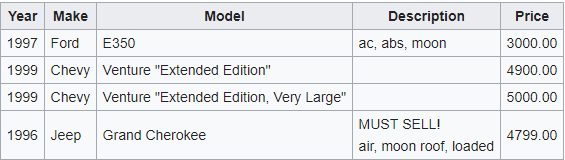
\includegraphics[width=0.6\textwidth]{figures/4/1174083/Teori/contohCSV1.png}}
		\caption{Contoh file}
		\label{Contoh CSV}
		\centerline{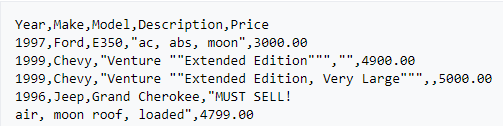
\includegraphics[width=0.6\textwidth]{figures/4/1174083/Teori/contohCSV2.png}}
		\caption{Contoh CSV}
		\label{Contoh CSV2}
	\end{figure}
	
\subsection{Soal 2}	

\textbf{Macam-macam aplikasi CSV}
\begin{enumerate}
\item Program Spreadsheet

Seperti Microsoft Excel, Kspread, Staroffice Calc, OpenOffice Calc, Abacus, Gnumeric, WingZ, XESS.			
\item Texteditor

Seperti Notepad, Notepad++, Sublime, NetBeans, Adobe Dreamweaver, Visual Studio Code, dll 

\end{enumerate}

\subsection{Soal 3}

\textbf{menulis dan membaca file csv}

Sesuai namanya, data atau nilai yang terdapat pada file CSV satu dengan yang lain dipisahkan dengan karakter koma (,). Jika berganti baris, maka itu dianggap record baru. Tentu saja ada kondisi tertentu yang harus dipenuhi agar file Excel bisa disimpan dalam format CSV. Setidaknya ada tiga kondisi utama yang harus dipenuhi, yaitu:
	\begin{itemize}
	\item Data yang diolah di Excel hanya berupa teks atau angka.
	\item Tidak mengandung VBA{Visual Basic for Application}.
	\item Hanya terdiri dari satu sheet.
	\end{itemize}

Langkah untuk menyimpan file ke dalam format CSV cukup mudah, yaitu dengan memilih File $>$ Save As (Excel 2003 atau sebelumnya) atau dengan mengklik Microsoft Office Button $>$ Save As pada Excel 2007. Setelah itu pada kotak dialog yang muncul, pilihlah format CSV (Comma delimited) (*.csv) melalui drop-down Save as type.

\subsection{Soal 4}

\textbf{Sejarah library CSV}

CSV digunakan pada tahun 1983. untuk komputer Osborne Executive, yang membundel spreadsheet SuperCalc, mendokumentasikan konvensi kutipan CSV yang memungkinkan string mengandung koma yang disematkan, tetapi manual tersebut tidak menentukan konvensi untuk menanamkan tanda kutip dalam string yang dikutip. Daftar nilai yang dipisahkan dengan koma lebih mudah untuk diketik daripada data yang selaras dengan kolom tetap, dan cenderung menghasilkan hasil yang salah jika suatu nilai dieksekusi satu kolom dari lokasi yang dituju.

\subsection{Soal 5}

\textbf{Sejarah library Pandas}

Pengembangnya ialah Wes McKinney, mulai mengerjakan pandas pada 2008 ketika di AQR Capital Management karena kebutuhan akan alat kinerja tinggi yang fleksibel untuk melakukan analisis kuantitatif pada data keuangan. Sebelum meninggalkan AQR, dia bisa meyakinkan manajemen untuk mengizinkannya membuka sumber perpustakaan. Pegawai AQR lainnya, Chang She, bergabung dengan proyek ini pada 2012 sebagai kontributor utama kedua ke perpustakaan. Pada 2015, pandas menandatangani sebagai proyek NumFOCUS yang disponsori secara fiskal, sebuah badan amal nirlaba 501(c)(3) di Amerika Serikat.

\subsection{Soal 6}

\textbf{Fungsi-fungsi pada library CSV}

\begin{itemize}
\item csv.reader

Berfungsi untuk membaca dan mengembalikan data kedalam variable dari file csv.	Fungsi 	reader dirancang untuk mengambil data pada setiap baris didalam file dan membuat daftar semua 	kolom. Kemudian, tinggal dipilih kolom mana yang diinginkan untuk data variabel.
\lstinputlisting[firstline=12, lastline=24]{src/4/1174083/Teori/1174083_csv.py}

\item csv.writer

Berfungsi untuk menuliskan data dari variable kedalam file csv. Fungsi writer akan membuat objek yang cocok untuk menulis. Untuk mengulang data yang ada di atas baris, gunakan fungsi writerow.
\lstinputlisting[firstline=39, lastline=45]{src/4/1174083/Teori/1174083_csv.py}
	
\item csv.register\textunderscore dialect untuk Mendaftarkan dialect pada csv
\item csv.unregister\textunderscore dialect untuk Menghapus dialect yang diasosiasi dengan nama dari registry dialect
\item csv.list\textunderscore dialects untuk Mengembalikan dialect yang diasosiasi dengan nama
\item csv.field\textunderscore size\textunderscore limit Mengembalikan ukuran field maksimum yang diizinkan oleh parser.
\item csv.DictReader

Berfungsi untuk membaca dan mengembalikan data kedalam variable dictionary dari file csv.
\lstinputlisting[firstline=26, lastline=37]{src/4/1174083/Teori/1174083_csv.py}
\end{itemize}

\subsection{Soal 7}

\textbf{•}

\begin{itemize}
\item pandas.read\textunderscore csv

Berfungsi untuk membaca dan mengembalikan data kedalam format DataFrame dari file csv.
\lstinputlisting[firstline=47, lastline=50]{src/4/1174083/Teori/1174083_csv.py}
\item to\textunderscore csv

Berfungsi untuk mengedit data didalam csv dan menulisnya kedalam file csv
\lstinputlisting[firstline=52, lastline=59]{src/4/1174083/Teori/1174083_csv.py}

\end{itemize}


\subsection{Bukti Screenshoot}
\begin{figure}[H]
	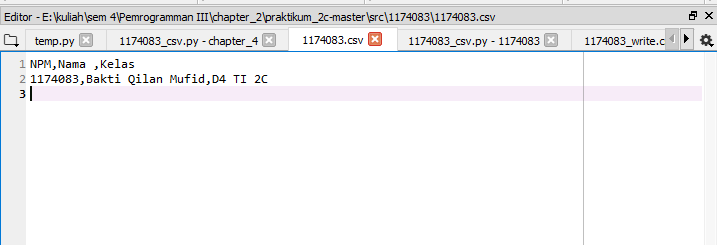
\includegraphics[width=10cm]{figures/4/1174083/Teori/kode_teori_1.png}
	\centering
\end{figure}

\begin{figure}[H]
	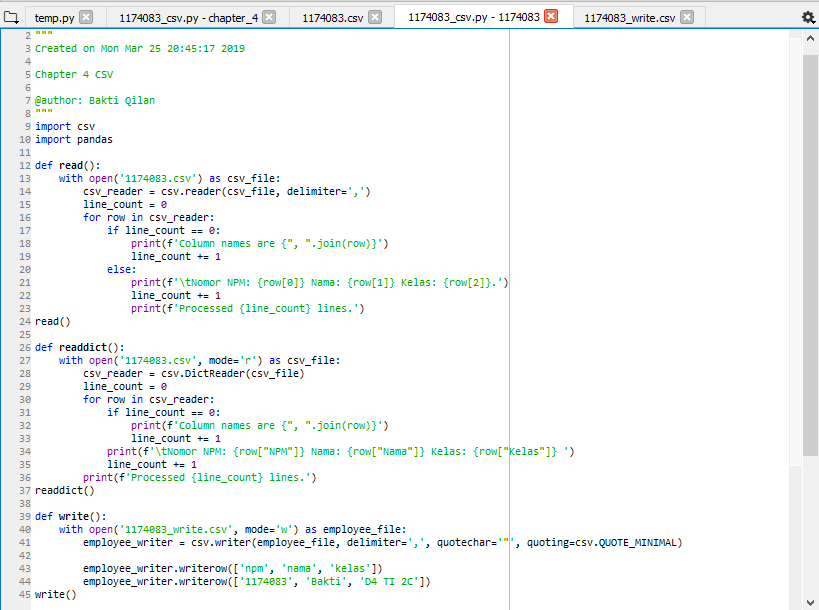
\includegraphics[width=10cm]{figures/4/1174083/Teori/kode_teori_2.png}
	\centering
\end{figure}

\begin{figure}[H]
	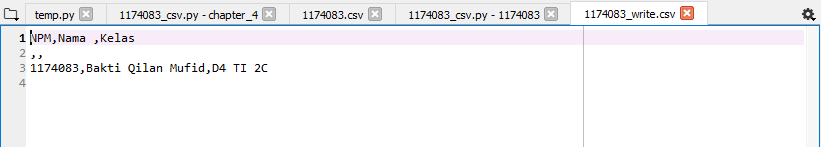
\includegraphics[width=10cm]{figures/4/1174083/Teori/kode_teori_3.png}
	\centering
\end{figure}

\begin{figure}[H]
	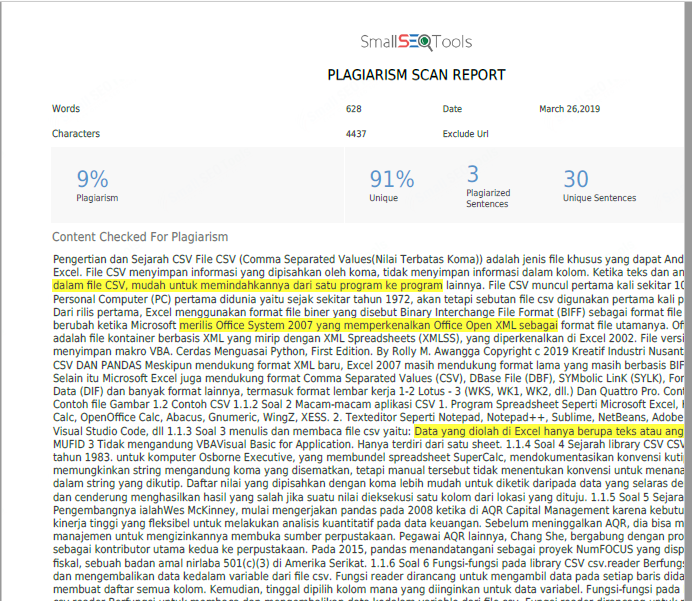
\includegraphics[width=10cm]{figures/4/1174083/Teori/plagiarisme.png}
	\centering	
	\caption{Cek Plagiat}
\end{figure}

%%%%%%%%%%%%%%%%%%%%%%%%%%%%%%%%%%%%%%%%%%%%%%%%%%%%%%%%%%%%%%%%%%%%%%%%%%%%%

\section{Muhammad Reza Syachrani / 1174084}
\subsection{Pemahaman Teori}
\begin{enumerate}
    \item CSV adalah Comma Separated Values suatu format data dalam basis data di mana setiap record dipisahkan dengan tanda koma (,) atau titik koma (;). Selain sederhana, format ini dapat dibuka dengan berbagai text-editor seperti Notepad, Wordpad, bahkan MS Excel.
    \par File CSV (Nilai Berbatas Koma) adalah tipe file khusus yang dapat Anda buat atau edit di Excel. File CSV menyimpan informasi yang dipisahkan oleh koma, bukan menyimpan informasi dalam kolom. Saat teks dan angka disimpan dalam file CSV, mudah untuk memindahkannya dari satu program ke program lain. Misalnya, Anda dapat mengekspor kontak dari Google ke dalam file CSV, kemudian mengimpornya ke Outlook.
    \item Aplikasi-aplikasi yang bisa menciptakan file CSV antara lain adalah notepad++, visual studio code, atom, sublime, excell, google spreadshare, dan LibreOfficecalc.
    \item Cara menulis file csv di excel atau spreadsheet
    \begin{enumerate}
        \item Buat dokumen baru di Excel.
        \item Tambahkan judul kolom untuk setiap informasi yang mau dicatat (misalnya nama, alamat email, nomor telepon, dan ulang tahun), selanjutnya ketikkan informasi dalam kolom yang sesuai.
        \item Setelah selesai, Pilih File > Simpan Sebagai.
        \item Gunakan kotak menurun untuk memilih CSV (Berbatas koma) (*.csv), beri nama pada file, lalu pilih Simpan
    \end{enumerate}
    \par Sedangkan cara membaca file csv di excel atau spreadsheet
    \begin{enumerate}
        \item klik data - get external data - form text
        \item Text Import Wizard, arahkan pada file csv lalu Open
        \item Setelah File terbuka, akan muncul Text Import Wizard.
        \item Pilih Delimited, Kemudian Next (Di sini, bisa juga menentukan baris awal yang akan di import)
        \item Centrang pada Tab dan Comma (Atau sesuai pengaturan File Anda) lalu Next.
        \item Atur Format data pada tiap kolom yang tampil dan klik Finish
    \end{enumerate}
    \item Sejarah Library CSV  dibuat untuk mepermudah mengolah data dan mempermudah untuk melakukan export dan import file CSV.
    \item Sejarah library pandas dibuat untuk bahasa pemograman python agar bisa bersaing dengan  R dan matlab, yang digunakan untuk mengolah banyak data , keperluan big data, data mining, dan data science.
    \item fungsi-fungsi yang terdapat di library CSV
    \begin{itemize}
        \item Reading CSV
        \par csv.reader digunakan untuk Membaca dari file CSV dilakukan menggunakan objek pembaca. File CSV dibuka sebagai file teks dengan fungsi open () built-in Python, yang mengembalikan objek file.
        \item Writing CSV
        \par csv.writer digunakan untuk dapat menulis ke file CSV.
    \end{itemize}
    \item fungsi-fungsi yang terdapat di library pandas
    \begin{itemize}
        \item Reading CSV
        \par pandas.read\_csv digunakan untuk membuka, menganalisis, dan membaca file CSV yang disediakan, dan menyimpan data dalam DataFrame.
        \item Writing CSV
        \par  Menulis DataFrame ke file CSV semudah membaca. contoh membuat variabel df yang menggunakan pandas.read\_csv setelah itu menambahkan fungsi to\_csv () pada varibel df untuk memberikan nama file.
    \end{itemize}
    
\end{enumerate}
\textbf{ Plagiarism}

\begin{figure}[H]
 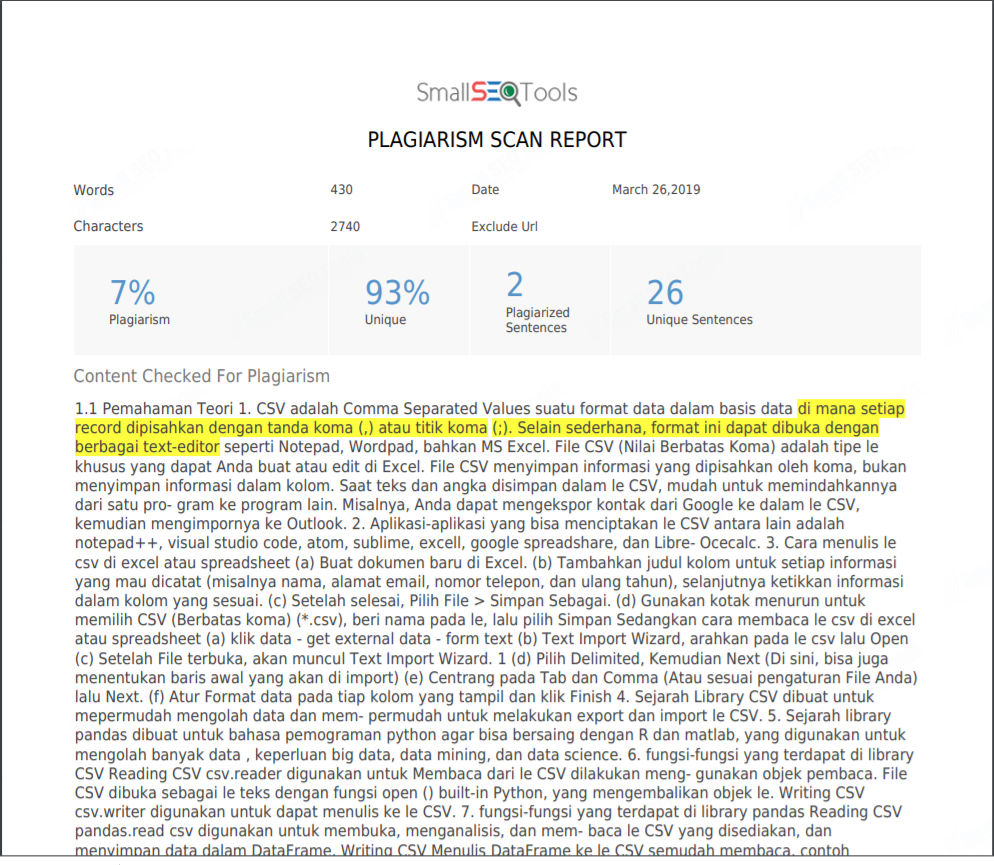
\includegraphics[width=10cm]{figures/4/1174084/Teori/c4_1.png}
 \centering
\end{figure}

%%%%%%%%%%%%%%%%%%%%%%%%%%%%%%%%%%%%%%%%%%%%%%%%%%%%%%%%%%%%%%%%%%%%%%%%%%%%%%